\subsection{Path Planning}
The path planning consist of two actions, finding a path with A\text{*} and then calculating coordinate targets in the map. 
A\text{*} uses a know map, an initial position, the goal and a cost map to plan out the path to the goal. 
The internal functionality of the A\text{*} function generates a heuristic map based on the goal and the know map.
The cost map is made so that all walls have a cost of 59, the grid cells less than 18 cm. from the walls have a cost of 9 and the rest of the grid cells have a cost of 1. The specific values have no real concern, but the walls have to have a high cost, preferable infinite, so that the robot does not plan on going through them. The area close to the wall are bad to be in, but not impossible to go through, so the value in these cells are higher than the cells further away. A dilation technique with a square structuring element was used to make the area that was close to the walls.
The implementation of A\text{*} is based upon the implementation from the Artificial Intelligence in Robotics Udacity course\citep{AIROK}.\\
The output of the A\text{*} is a path and a policy vector. The policy vector is used to calculate some coordinate targets which are used as targets when the robot moves towards the goal. An example of a plan can be seen in figure \ref{fig:exastar} where start is [ 1 1 ] and the goal is [ 6 5 ]. For a real world example see the results section.
\begin{figure}[H]
\centering
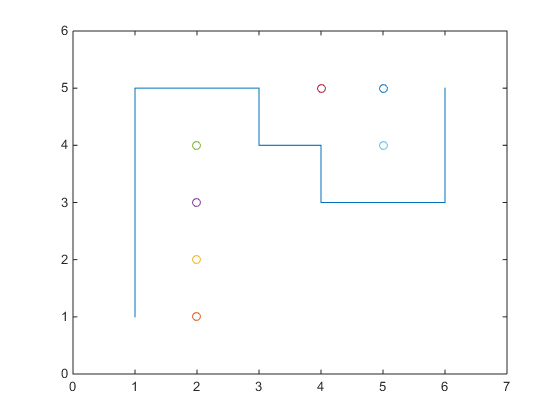
\includegraphics[width=0.5\textwidth]{billeder/exampleastar}
\caption{Example of A star plan}
\label{fig:exastar}
\end{figure}